\documentclass[12pt,a4paper]{article}
\usepackage[utf8]{inputenc}
\usepackage[T1]{fontenc}
\usepackage{graphicx}
\usepackage{amsmath}
\usepackage[margin=2.5cm]{geometry}

\title{Oscilloscopes and Function Generators}
\author{Terje\\
        \texttt{	
terje.frisse@uni-oldenburg.de}\\Ayoub\\\texttt{ayoub.jaziri@uni-oldenburg.de}\\Group 7}
\date{\today}
\usepackage{float}
\usepackage{graphicx}
\begin{document}
\maketitle

\begin{abstract}
In this report, we learned how to measure with a digital oscilloscope (OSC)
and how to generate test signals with a function generator (FG). We
displayed signals of different shapes, changed the trigger settings, and used
the measurement functions of the OSC to read off amplitudes, frequencies and
time differences. We also recorded signals from a photodetector, among them
a single light flash, whose duration was found to be
$t_b = (380 \pm 50)~\mu$s. This value is only an upper limit, because we
forgot the 50~$\Omega$ termination of the detector.
\end{abstract}

\section{Introduction}
An oscilloscope (OSC) records a voltage $U$ and shows how it changes with
time $t$. With suitable sensors, such as a photodetector, it can display
many other quantities as well. A function generator (FG) provides the
voltage signals that are used to test and calibrate such measurements. In
this report we use both devices to get familiar with their main functions.

\section{Experiments}
\subsection{Duration of a Light Flash}
This experiment was aimed at determining the duration of a light flash using a photodetector and an OSC. Therefore, the voltage signal of the detector, which follows the light intensity of a single flash, was recorded in single-sequence mode, and the 10\%-width $t_b$ of the pulse was evaluated.

\subsubsection{Method}
The output of the photodetector was connected to channel 1 of the OSC with a coaxial cable. A block diagram of the setup is shown in Fig.~\ref{fig:setup}. The flash was directed at the detector from a distance of about [0.5--1]~m. The OSC was triggered on the rising edge in single-sequence mode. No 50~$\Omega$ termination was used. The duration is defined as the 10\%-width $t_b$, i.e., the time between the rising and falling crossings of $0.1\,U_0$, where $U_0$ is the pulse amplitude.

\begin{figure}[htbp]
  \centering
 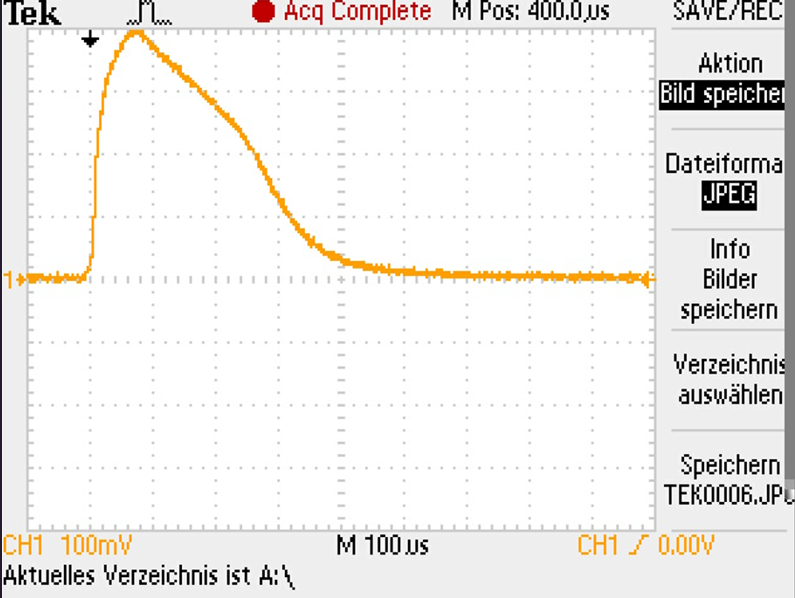
\includegraphics[width=0.6\textwidth]{TEK0006.png}
  \caption{Block diagram of the setup: photodetector connected directly to the OSC input.}
  \label{fig:setup}
\end{figure}

\subsubsection{Results and Discussion}
The recorded pulse is shown in Fig.~\ref{fig:flash}. It has a fast rise and a slow decay. The amplitude is $U_0 \approx 0.40$~V, so $0.1\,U_0 \approx 0.04$~V. The values are listed in Tab.~\ref{tab:flash}. The duration is $t_b = (380 \pm [50])~\mu$s.

\begin{table}[htbp]
  \centering
  \caption{Pulse amplitude, 10\% level and 10\%-width of the flash pulse.}
  \label{tab:flash}
  \begin{tabular}{ll}
    \hline
    Quantity & Value \\
    \hline
    $U_0$ / V & $0.40 \pm [0.02]$ \\
    $0.1\,U_0$ / V & $0.040 \pm [0.002]$ \\
    $t_b$ / $\mu$s & $380 \pm [50]$ \\
    \hline
  \end{tabular}
\end{table}

\begin{figure}[H]
  \centering
  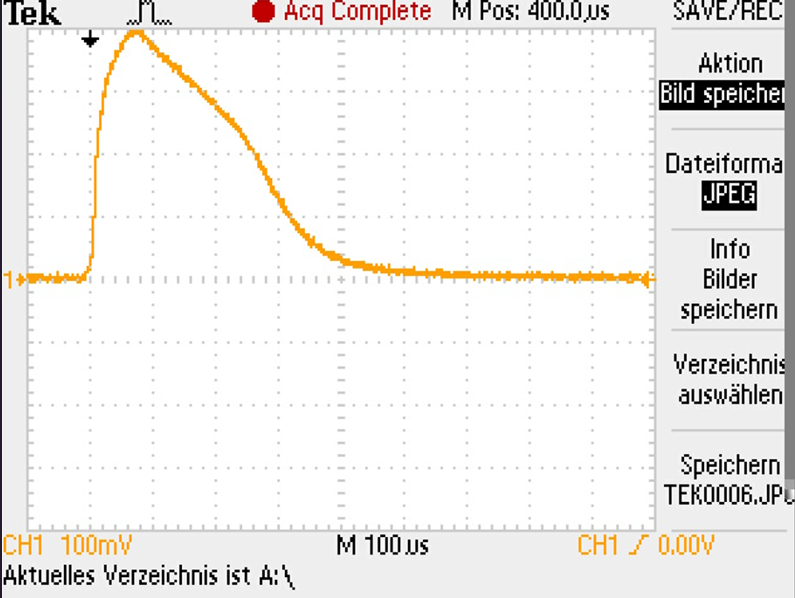
\includegraphics[width=0.8\textwidth]{TEK0006.png}
  \caption{Voltage $U(t)$ of the photodetector for a single flash without 50~$\Omega$ termination (100~$\mu$s/div, 100~mV/div).}
  \label{fig:flash}
\end{figure}

Without the 50~$\Omega$ termination, the oscilloscope input resistance ($R_o \approx 1$~M$\Omega$) and the capacitance $C$ of the input and the cable form a low-pass filter with the time constant $\tau = R_o C$. With an estimated $C \approx 100$~pF, we get $\tau \approx 100~\mu$s. The signal needs about $2.3\,\tau \approx 230~\mu$s to fall to 10\%, which is of the same order as $t_b$. The measured $t_b$ is therefore an upper limit for the real flash duration. With a 50~$\Omega$ resistor, $\tau$ would be about 5~ns.
\section{Results and Discussion}
% \begin{figure}[h]
%   \centering
%   \includegraphics[width=0.7\textwidth]{plot.png}
%   \caption{Measured signal.}
% \end{figure}

\section{Conclusion}
Summarise your findings.

\begin{thebibliography}{9}
\bibitem{ref1} Author, \textit{Title of Book}, Publisher, Year.
\end{thebibliography}

\end{document}